\subsection{Attention and Transformer} % 2.5 pages
The attention mechanism originated from the human experience of perceiving things either visually or audibly.
Intuitively speaking, when we observe something through sight, we do not pay attention to all the details but paying attention to a certain part that needs to be focused and giving low attention to the surroundings.

The attention mechanism was firstly added to recurrent neural networks as a visual attention modelling.
In 2014, \citet{mnih2014recurrent} proposed a recurrent attention model that combined ideas in RNN and the attention mechanism for image classification and achieved good performance.
Besides, the researchers discussed and reached forward-looking conclusions that it can be used in object recognition and video classification in future work due to the encouraging results achieved.

In 2016, \citet{bahdanau2016neural} firstly introduced the attention mechanism into the natural language processing field.
In their work, they perform translation and alignment jointly with the attention mechanism on machine translation tasks because ``the use of a fixed-length vector is a bottleneck in improving the performance of this basic encoder-decoder architecture'', said by \citet{bahdanau2016neural}.

\begin{minipage}[]{\textwidth}
\centering
\begin{minipage}[ht]{.35\textwidth}
    \centering
    \begin{figure}[H]
        \centering
        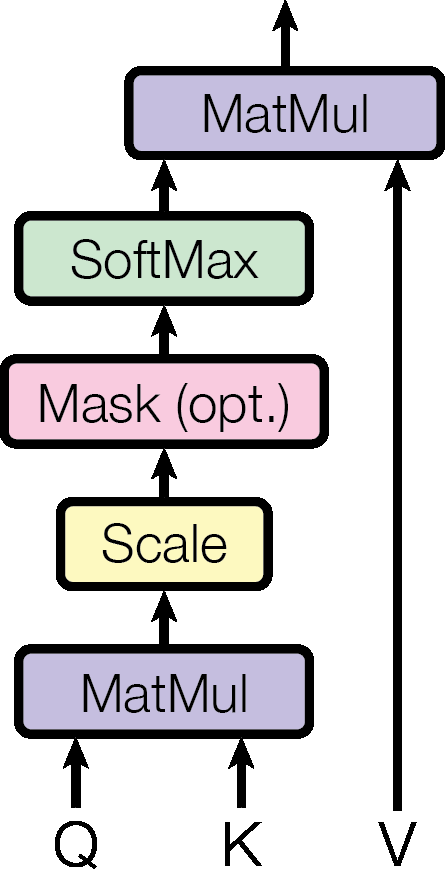
\includegraphics[width=.48\textwidth]{literature/imgs/ext-attention-dot-product.png}
        \caption{Scaled Dot-Product Attention \cite{vaswani2017attention}}
        \label{fig:ext-attention-dot-product}
    \end{figure}
    \vspace*{-.5cm}
    \begin{figure}[H]
        \centering
        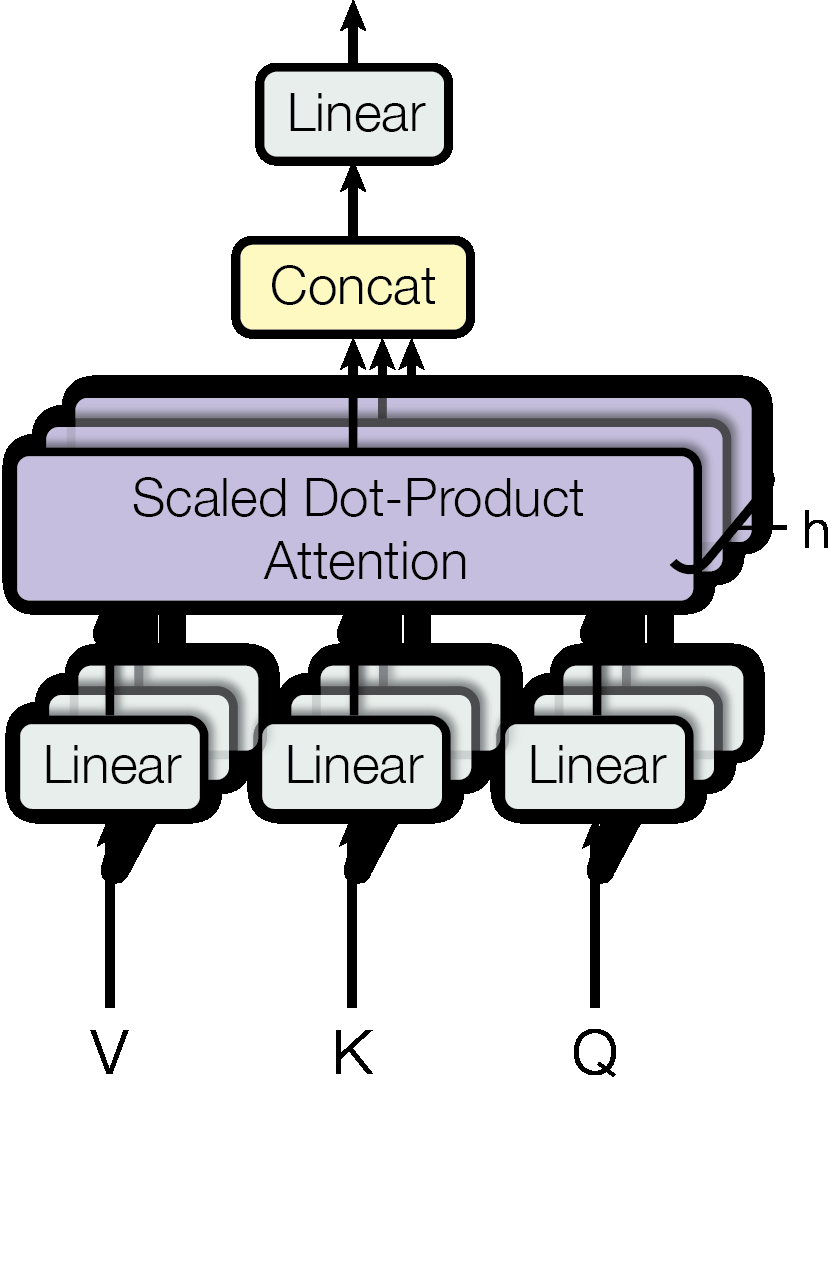
\includegraphics[width=.9\textwidth]{literature/imgs/ext-attention-multihead.png}
        \vspace*{-2em}
        \caption{Multi-Head Attention \cite{vaswani2017attention}}
        \label{fig:ext-attention-multihead}
    \end{figure}
\end{minipage}
\hspace{1em}
\begin{minipage}[ht]{.52\textwidth}
    \begin{figure}[H]
        \centering
        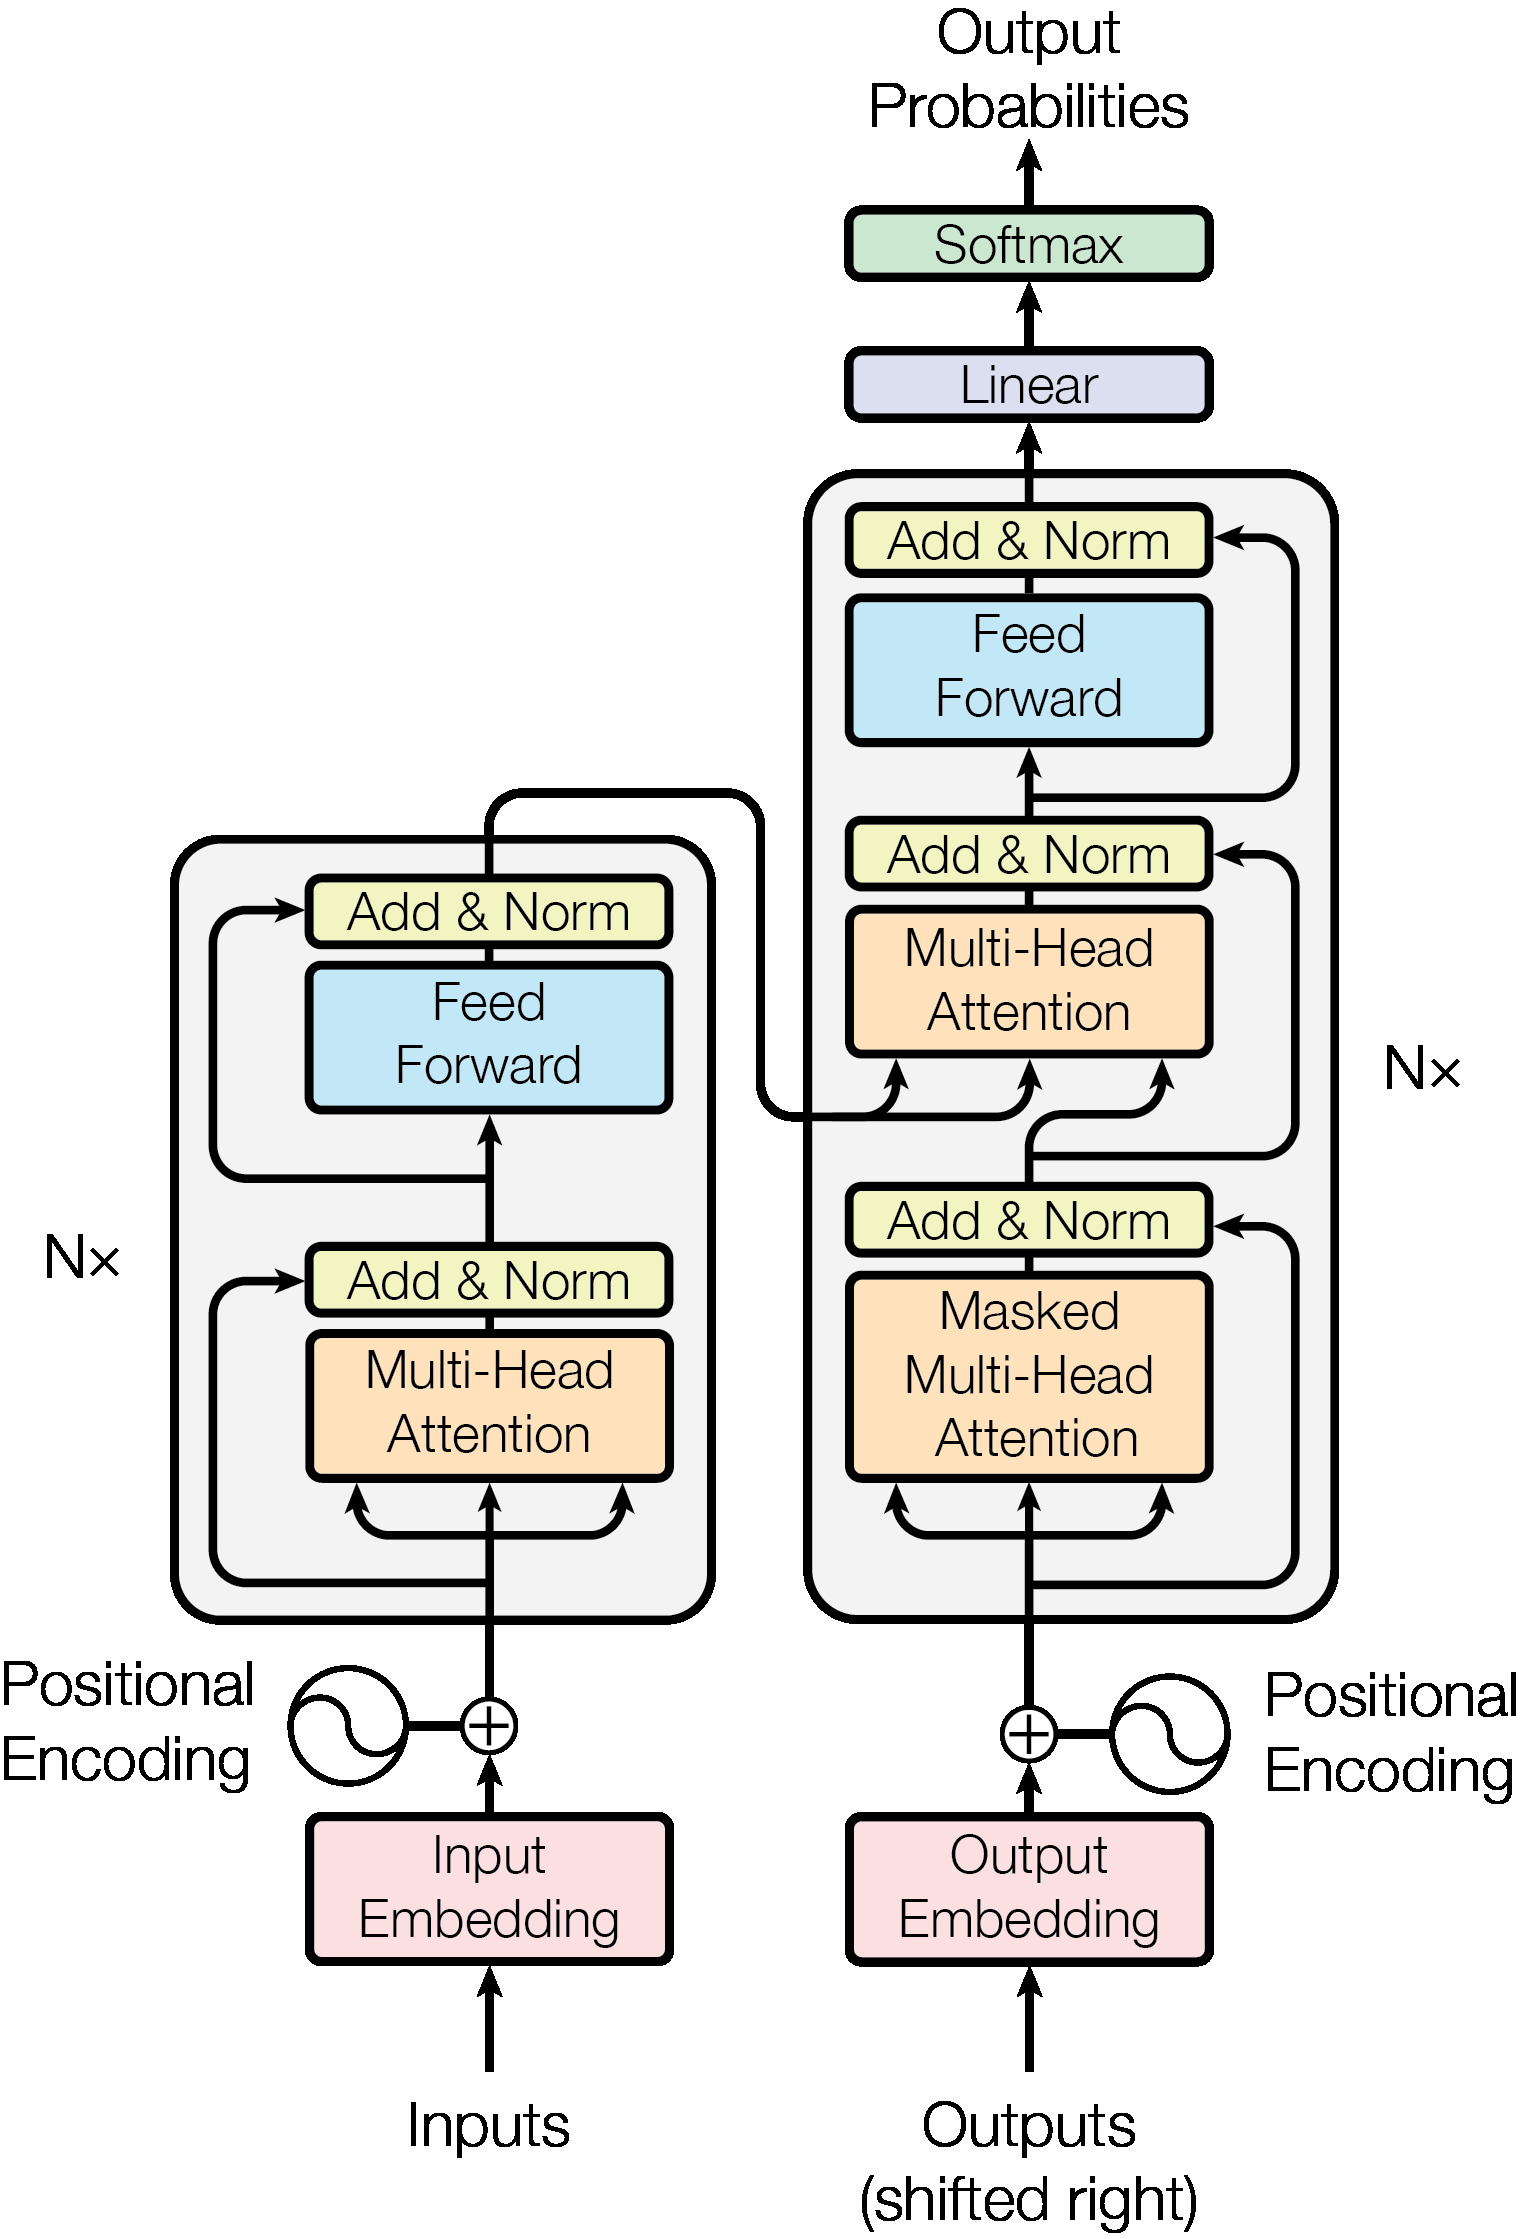
\includegraphics[width=\textwidth]{literature/imgs/ext-transformer.png}
        \caption{The Transformer model architecture \cite{vaswani2017attention}}
        \label{fig:ext-transformer}
    \end{figure}
\end{minipage}
\end{minipage}

One year after the attention mechanism was applied in the machine translation tasks, \citet{vaswani2017attention} proposed scaled dot-product attention (Figure \ref{fig:ext-attention-dot-product}), multi-head attention (Figure \ref{fig:ext-attention-multihead}) and the Transformer model (Figure \ref{fig:ext-transformer}) that is ``relying entirely on self-attention to compute representations of its input and output without using sequence aligned RNNs or convolution'', said by \citet{vaswani2017attention}.
Then, experiments were performed on the machine translation task using the proposed Transformer model and achieved better performance and results, making the attention mechanism the most preferred solution for natural language processing tasks.

\begin{equation}
    Attention(Q, K, V) = softmax(\frac{QK^T}{\sqrt{d_k}})V
    \eqcite{vaswani2017attention}
    \label{eq:2-attention}
\end{equation}

Figure \ref{fig:ext-attention-dot-product} shows the scaled dot-product attention mechanism, where Q, K, and V represent Query, Key and Value respectively.
Further, formula \ref{eq:2-attention} shows the calculation process of it mathematically.
In this formula, the dot-product between Query and Key matrix represents their similarity, which is normalised by the square root of the dimension of $d_k$, since dot-product may grow large in magnitude, pushing the softmax activation function into regions where it has extremely small gradients.
The result from softmax activation is normalised probabilities representing the attention matrix visualised in Figure  \ref{fig:ext-attention_map_portuguese}.

\begin{figure}[!ht]
    \centering
    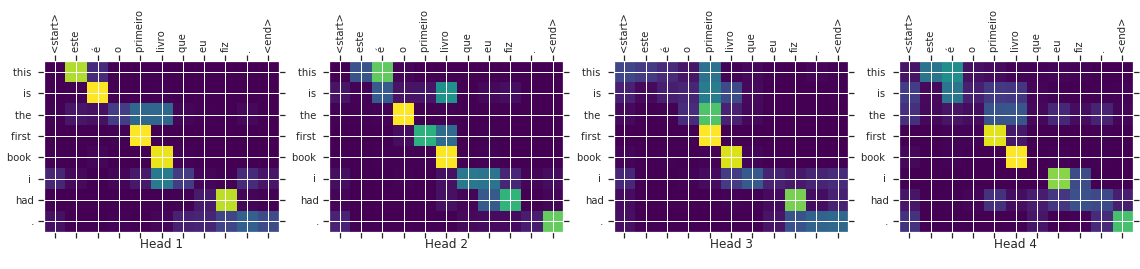
\includegraphics[width=\textwidth]{literature/imgs/ext-attention_map_portuguese.png}
    \caption{Multi-head attention matrix visualisation \cite{tensorflow2021transformer}}
    \label{fig:ext-attention_map_portuguese}
\end{figure}

The idea behind multi-head attention is analogous in using multiple kernel filters in CNN to help the network capture richer feature sub-spaces on different aspects of data.
Figure \ref{fig:ext-attention-multihead} illustrates the structure of the multi-head attention. It contains linear layers at inputs and the output, $h$ times the scaled dot-product attention computation process, and a concatenation layer that combines the outputs of each scaled dot-product attention.

The building block in the Transformer consists only of multi-head attention and feed-forward network and does not contain any convolution or recurrent structure.
These building blocks are stacked in multiple layers and connected in residuals to form an Encoder-Decoder structure that is the Transformer model shown in Figure \ref{fig:ext-transformer}.

Another detail worth mentioning in the Figure \ref{fig:ext-transformer} is that the input content needs to add position encoding because this model is not sequential input, which implicitly includes position information.
If there is no positional encoding added, Transformer will not be able to capture the order of input sequence, which degenerates it into a bag-of-words model in natural language processing tasks.

While convolutional neural network (CNN) is in the ascendant among the fields of computer vision, the Transformer model composed of pure attention mechanism has achieved state-of-the-art results in many natural language processing tasks.

In 2018, \citet{devlin2019bert} published the Bidirectional Encoder Representations from Transformers (BERT) model, in which the Mask Language Model (MLM) and Next Sentence Prediction (NSP), two methods are used in the pre-training process to make Transformers capture the relationship between words and sentences.
The amazing results in many NLP tasks from this model became the most important contribution that started a new era of NLP in 2018.

As a result, the Transformer model gradually replaced the RNN-based seq2seq model that inherently has sequential computing and long-term memory loss issues. Innovative design concepts from the Transformer model are also carried forward from the fields of natural language processing to computer vision territory.

\begin{wrapfigure}{l}{0.5\textwidth}
    \vspace*{-1em}
    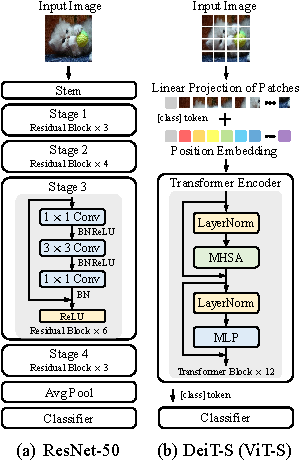
\includegraphics[width=.5\textwidth]{literature/imgs/ext-res50-deit-s.pdf}
    \caption{Compare the architecture of ResNet-50 and DeiT-S (ViT-S)\cite{guo2021cmt}}
    \label{fig:ext-res50-deit-s}
\end{wrapfigure}

Recent studies are exploring the application of Transformers architecture in the field of computer vision recently, such as Data-efficient image Transformers (DeiT) and Shifted window (Swin) Transformers.
Many researchers have tried to introduce the attention mechanism in imagery tasks and compared model designs and results with widely-adopted CNN-only models such as ResNet, illustrated in Figure \ref{fig:ext-res50-deit-s}.

However, \citet{dai2021coatnet} pointed out that the performance of Transformers-based vision models still has a gap compared with state-of-the-art convolutional networks.
They also showed that the generalisation is worse than convolutional networks because of the lack of the right inductive bias in the Transformers-based vision models.
As a result, they proposed a hybrid model that married convolution and attention, leading the future research direction from this attempt.